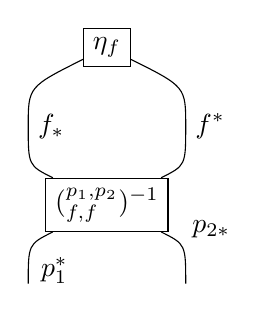
\begin{tikzpicture}[baseline=(current bounding box.center),]
\path coordinate[] (tikzsd_internal_pos_1_0) at (0.0,-2.0);
\path coordinate[] (tikzsd_internal_pos_1_1) at (2.0,-2.0);
\path coordinate[] (tikzsd_internal_pos_2_0) at (0.0,-4.0);
\path coordinate[] (tikzsd_internal_pos_2_1) at (2.0,-4.0);

\path node[,draw,] (tikzsd_internal_nt_node_0_0) at (1.0,-1.0) {$\eta_f$};
\path node[,draw,] (tikzsd_internal_nt_node_1_0) at (1.0,-3.0) {$(\PP_{f,f}^{p_1,p_2})^{-1}$};

\path [draw] (tikzsd_internal_nt_node_0_0) ..controls(0.0,-1.5)..(tikzsd_internal_pos_1_0) ..controls(0.0,-2.5)..(tikzsd_internal_nt_node_1_0) node[pos=0.0,auto,] {$f_\ast$};
\path [draw] (tikzsd_internal_nt_node_0_0) ..controls(2.0,-1.5)..(tikzsd_internal_pos_1_1) ..controls(2.0,-2.5)..(tikzsd_internal_nt_node_1_0) node[pos=0.0,auto,] {$f^\ast$};
\path [draw] (tikzsd_internal_nt_node_1_0) ..controls(0.0,-3.5)..(tikzsd_internal_pos_2_0) node[pos=0.5,auto,] {$p_1^\ast$};
\path [draw] (tikzsd_internal_nt_node_1_0) ..controls(2.0,-3.5)..(tikzsd_internal_pos_2_1) node[pos=0.5,auto,] {$p_{2\ast}$};
\end{tikzpicture}